% Q09 -- 3T DRAM cell STICK diagram (simplified, colour-coded layers).
% poly = red (WL, RL gates), n-diffusion = green (M1 write, M2 read-evaluate, M3 read-access),
% metal = blue (BL, BLbar bit lines + storage node X), contacts = black squares.
\documentclass[border=10pt]{standalone}
\usepackage{tikz}
\begin{document}
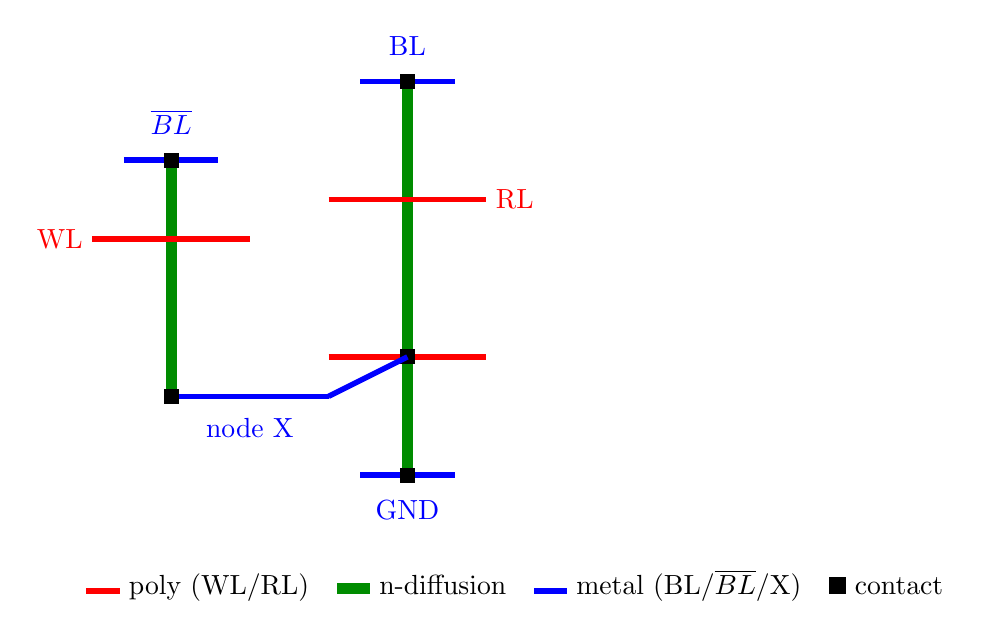
\begin{tikzpicture}[
  poly/.style={red, line width=2pt},
  ndiff/.style={green!55!black, line width=4pt},
  metal/.style={blue, line width=2pt},
  cont/.style={fill=black, draw=black, minimum size=5pt, inner sep=0pt}]
% ---- write branch (left): M1 diffusion, WL poly, BLbar metal ----
\draw[ndiff] (1,2) -- (1,5);            % M1 diffusion
\draw[poly]  (0,4) -- (2,4);            % WL poly = gate of M1
\node[left, red] at (0,4) {WL};
\draw[metal] (0.4,5) -- (1.6,5);        % BLbar metal at top of M1
\node[above, blue] at (1,5.2) {$\overline{BL}$};
\node[cont] at (1,5) {};
% ---- storage node X : metal link from M1 to gate poly of M2 ----
\draw[metal] (1,2) -- (3,2);
\node[below, blue] at (2,1.85) {node X};
\node[cont] at (1,2) {};
% ---- read branch (right): M2 (read-eval) + M3 (read-access) in series ----
\draw[ndiff] (4,1) -- (4,6);            % shared read diffusion (M2 then M3)
\draw[poly]  (3,2.5) -- (5,2.5);        % gate of M2 driven by node X
\node[cont] at (4,2.5) {};              % X contacts M2 gate poly
\draw[metal] (3,2) -- (4,2.5);          % X metal up to M2 gate
\draw[poly]  (3,4.5) -- (5,4.5);        % RL poly = gate of M3
\node[right, red] at (5,4.5) {RL};
% read bit line (metal) at top of the series branch
\draw[metal] (3.4,6) -- (4.6,6);
\node[above, blue] at (4,6.2) {BL};
\node[cont] at (4,6) {};
% bottom of read branch to ground rail (metal)
\draw[metal] (3.4,1) -- (4.6,1);
\node[below, blue] at (4,0.8) {GND};
\node[cont] at (4,1) {};
% legend
\node[anchor=west, align=left] at (-0.2,-0.4)
 {\textcolor{red}{$\rule{12pt}{2pt}$} poly (WL/RL)\quad
  \textcolor{green!55!black}{$\rule{12pt}{4pt}$} n-diffusion\quad
  \textcolor{blue}{$\rule{12pt}{2pt}$} metal (BL/$\overline{BL}$/X)\quad
  \rule{6pt}{6pt}~contact};
\end{tikzpicture}
\end{document}
